\begin{enumerate}[\bf 1.]
	\item[]
	\begin{figure}[h!]\centering
		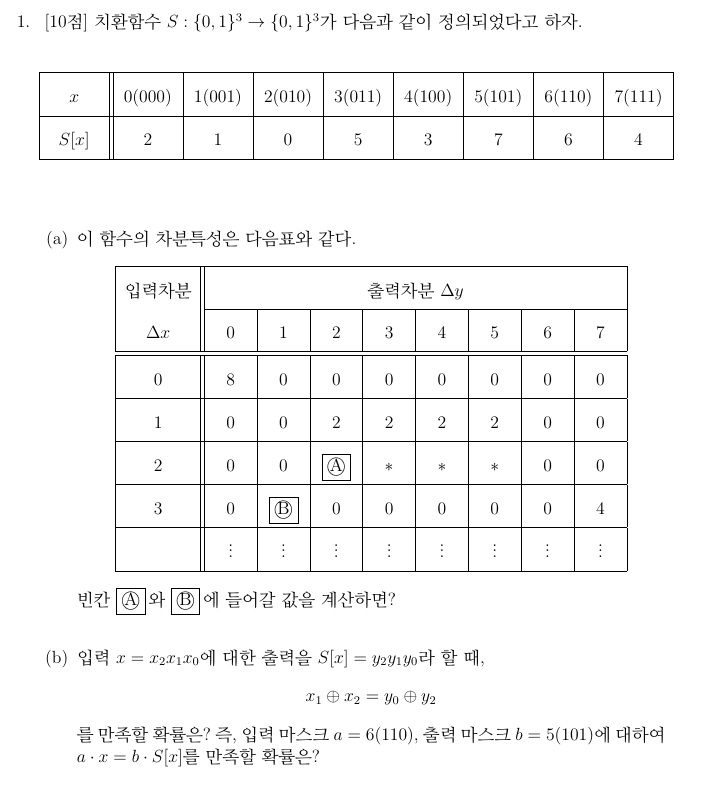
\includegraphics[scale=.525]{final2023-1}
	\end{figure}
	\begin{proof}[\sol]
		\begin{enumerate}[(a)]
			\item $A=2$ and  $B=4$: \begin{center}
				\begin{tabular}{cc|cc|c}
					\toprule[1.2pt]
					$x$ & $x \oplus 010$ & $S[x]$ & $S[x\oplus 010]$ & $\Delta y$\\ \hline
					000 & 010 & 010 & 000 & 010 \\
					001 & 011 & 001 & 101 & 100 \\
					010 & 000 & 000 & 010 & 010 \\
					011 & 001 & 101 & 001 & 100 \\
					100 & 110 & 011 & 110 & 101 \\
					101 & 111 & 111 & 100 & 011 \\
					110 & 100 & 110 & 011 & 101 \\
					111 & 101 & 100 & 111 & 011 \\
					\bottomrule[1.2pt]
				\end{tabular}$\implies$ $P[\Delta x=2\to\Delta y=2]=2/8=1/4$.
			\end{center}
			\item \ \begin{table}[h!]\centering
				\begin{tabular}{ccc|ccc|cc}
					\toprule[1.2pt]
					\textcolor{red}{$[x_2]$} & \textcolor{red}{$[x_1]$} & $x_0$ & \textcolor{red}{$[y_2]$} & {$y_1$} & \textcolor{red}{$[y_0]$} & $a\cdot x=b\cdot y$ & \\
					\hline
					0 & 0 & 0 & 0 & 1 & 0 & $0=0$ & \textcolor{green}{\checkmark}\\
					0 & 0 & 1 & 0 & 0 & 1 & $0=1$ & \textcolor{red}{\xmark}\\
					0 & 1 & 0 & 0 & 0 & 0 & $1=0$ & \textcolor{red}{\xmark}\\
					0 & 1 & 1 & 1 & 0 & 1 & $1=0$ & \textcolor{red}{\xmark}\\
					1 & 0 & 0 & 0 & 1 & 1 & $1=1$ & \textcolor{green}{\checkmark}\\
					1 & 0 & 1 & 1 & 1 & 1 & $1=0$ & \textcolor{red}{\xmark}\\
					1 & 1 & 0 & 1 & 1 & 0 & $0=1$ & \textcolor{red}{\xmark}\\
					1 & 1 & 1 & 1 & 0 & 0 & $0=1$ & \textcolor{red}{\xmark}\\
					\bottomrule[1.2pt]
				\end{tabular}$\implies$ the probability is $2/8=1/4$.
			\end{table}
		\end{enumerate}
	\end{proof}
	\item[]
	\begin{figure}[h!]\centering
		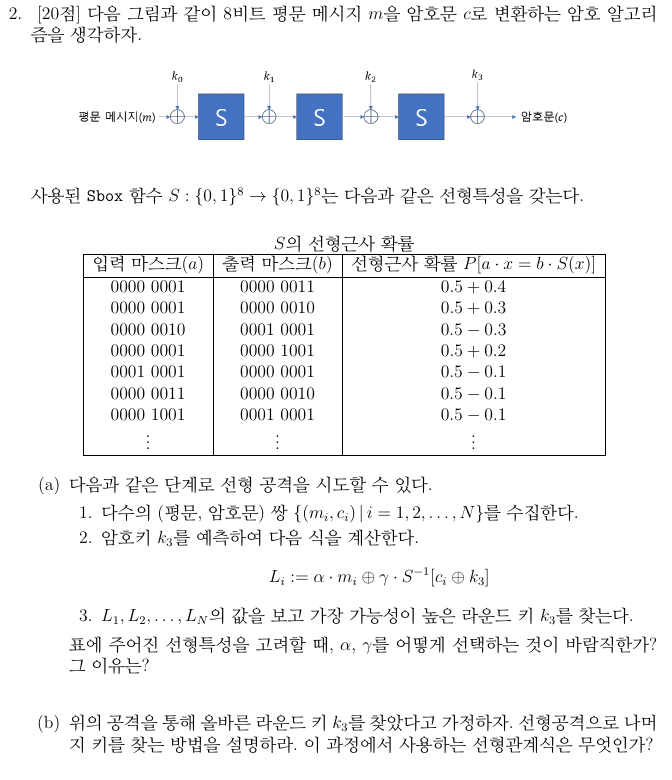
\includegraphics[scale=.57]{final2023-2}
	\end{figure}
	\begin{proof}[\sol]
		\ \\ \adjustbox{scale=1, center}{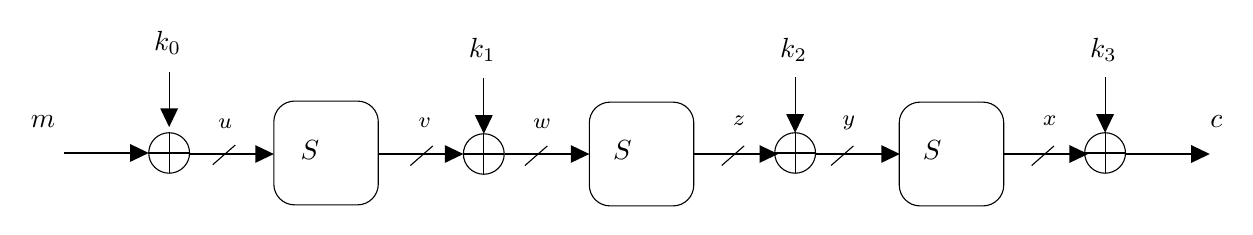
\begin{tikzpicture}[x=0.75pt,y=0.75pt,yscale=-1,xscale=1]
			%uncomment if require: \path (0,300); %set diagram left start at 0, and has height of 300	
			%Flowchart: Or [id:dp6387090213276583] 
			\draw   (114.73,150) .. controls (114.73,144.62) and (119.14,140.25) .. (124.57,140.25) .. controls (130,140.25) and (134.4,144.62) .. (134.4,150) .. controls (134.4,155.38) and (130,159.75) .. (124.57,159.75) .. controls (119.14,159.75) and (114.73,155.38) .. (114.73,150) -- cycle ; \draw   (114.73,150) -- (134.4,150) ; \draw   (124.57,140.25) -- (124.57,159.75) ;
			%Rounded Rect [id:dp2984270284803445] 
			\draw   (175,135) .. controls (175,129.48) and (179.48,125) .. (185,125) -- (215.33,125) .. controls (220.86,125) and (225.33,129.48) .. (225.33,135) -- (225.33,165) .. controls (225.33,170.52) and (220.86,175) .. (215.33,175) -- (185,175) .. controls (179.48,175) and (175,170.52) .. (175,165) -- cycle ;
			%Flowchart: Or [id:dp403217021780772] 
			\draw   (266.33,150.5) .. controls (266.33,145.12) and (270.74,140.75) .. (276.17,140.75) .. controls (281.6,140.75) and (286,145.12) .. (286,150.5) .. controls (286,155.88) and (281.6,160.25) .. (276.17,160.25) .. controls (270.74,160.25) and (266.33,155.88) .. (266.33,150.5) -- cycle ; \draw   (266.33,150.5) -- (286,150.5) ; \draw   (276.17,140.75) -- (276.17,160.25) ;
			%Rounded Rect [id:dp7969101552713898] 
			\draw   (327,135.5) .. controls (327,129.98) and (331.48,125.5) .. (337,125.5) -- (367.33,125.5) .. controls (372.86,125.5) and (377.33,129.98) .. (377.33,135.5) -- (377.33,165.5) .. controls (377.33,171.02) and (372.86,175.5) .. (367.33,175.5) -- (337,175.5) .. controls (331.48,175.5) and (327,171.02) .. (327,165.5) -- cycle ;
			%Flowchart: Or [id:dp6677888640244123] 
			\draw   (416.33,150) .. controls (416.33,144.62) and (420.74,140.25) .. (426.17,140.25) .. controls (431.6,140.25) and (436,144.62) .. (436,150) .. controls (436,155.38) and (431.6,159.75) .. (426.17,159.75) .. controls (420.74,159.75) and (416.33,155.38) .. (416.33,150) -- cycle ; \draw   (416.33,150) -- (436,150) ; \draw   (426.17,140.25) -- (426.17,159.75) ;
			%Straight Lines [id:da5362001581563707] 
			\draw    (134.4,150.5) -- (155.67,150.5) -- (172,150.5) ;
			\draw [shift={(175,150.5)}, rotate = 180] [fill={rgb, 255:red, 0; green, 0; blue, 0 }  ][line width=0.08]  [draw opacity=0] (8.93,-4.29) -- (0,0) -- (8.93,4.29) -- cycle    ;
			%Straight Lines [id:da39216223723804444] 
			\draw    (225.73,150.5) -- (247,150.5) -- (263.33,150.5) ;
			\draw [shift={(266.33,150.5)}, rotate = 180] [fill={rgb, 255:red, 0; green, 0; blue, 0 }  ][line width=0.08]  [draw opacity=0] (8.93,-4.29) -- (0,0) -- (8.93,4.29) -- cycle    ;
			%Straight Lines [id:da17543897115899898] 
			\draw    (286.4,150.5) -- (307.67,150.5) -- (324,150.5) ;
			\draw [shift={(327,150.5)}, rotate = 180] [fill={rgb, 255:red, 0; green, 0; blue, 0 }  ][line width=0.08]  [draw opacity=0] (8.93,-4.29) -- (0,0) -- (8.93,4.29) -- cycle    ;
			%Straight Lines [id:da7242342168072087] 
			\draw    (377.33,150.5) -- (398.6,150.5) -- (414.93,150.5) ;
			\draw [shift={(417.93,150.5)}, rotate = 180] [fill={rgb, 255:red, 0; green, 0; blue, 0 }  ][line width=0.08]  [draw opacity=0] (8.93,-4.29) -- (0,0) -- (8.93,4.29) -- cycle    ;
			%Straight Lines [id:da10920614678319085] 
			\draw    (436,150.5) -- (457.27,150.5) -- (473.6,150.5) ;
			\draw [shift={(476.6,150.5)}, rotate = 180] [fill={rgb, 255:red, 0; green, 0; blue, 0 }  ][line width=0.08]  [draw opacity=0] (8.93,-4.29) -- (0,0) -- (8.93,4.29) -- cycle    ;
			%Straight Lines [id:da08748396717157081] 
			\draw    (74.13,150) -- (95.4,150) -- (111.73,150) ;
			\draw [shift={(114.73,150)}, rotate = 180] [fill={rgb, 255:red, 0; green, 0; blue, 0 }  ][line width=0.08]  [draw opacity=0] (8.93,-4.29) -- (0,0) -- (8.93,4.29) -- cycle    ;
			%Straight Lines [id:da4140953307861994] 
			\draw    (124.57,110.75) -- (124.57,122.75) -- (124.57,134.5) ;
			\draw [shift={(124.57,137.5)}, rotate = 270] [fill={rgb, 255:red, 0; green, 0; blue, 0 }  ][line width=0.08]  [draw opacity=0] (8.93,-4.29) -- (0,0) -- (8.93,4.29) -- cycle    ;
			%Straight Lines [id:da4902037387269014] 
			\draw    (276.17,114) -- (276.17,126) -- (276.17,137.75) ;
			\draw [shift={(276.17,140.75)}, rotate = 270] [fill={rgb, 255:red, 0; green, 0; blue, 0 }  ][line width=0.08]  [draw opacity=0] (8.93,-4.29) -- (0,0) -- (8.93,4.29) -- cycle    ;
			%Straight Lines [id:da032438173515496604] 
			\draw    (426.17,113.5) -- (426.17,125.5) -- (426.17,137.25) ;
			\draw [shift={(426.17,140.25)}, rotate = 270] [fill={rgb, 255:red, 0; green, 0; blue, 0 }  ][line width=0.08]  [draw opacity=0] (8.93,-4.29) -- (0,0) -- (8.93,4.29) -- cycle    ;
			%Straight Lines [id:da38705791074267304] 
			\draw    (156.38,146.21) -- (145.6,155.64) ;
			%Straight Lines [id:da6577256556176674] 
			\draw    (251.58,146.61) -- (240.8,156.04) ;
			%Straight Lines [id:da9791366655045883] 
			\draw    (306.78,146.61) -- (296,156.04) ;
			%Straight Lines [id:da12965720331903818] 
			\draw    (401.58,146.61) -- (390.8,156.04) ;
			%Rounded Rect [id:dp47562690354046877] 
			\draw   (476.33,135.5) .. controls (476.33,129.98) and (480.81,125.5) .. (486.33,125.5) -- (516.67,125.5) .. controls (522.19,125.5) and (526.67,129.98) .. (526.67,135.5) -- (526.67,165.5) .. controls (526.67,171.02) and (522.19,175.5) .. (516.67,175.5) -- (486.33,175.5) .. controls (480.81,175.5) and (476.33,171.02) .. (476.33,165.5) -- cycle ;
			%Flowchart: Or [id:dp5220437140255207] 
			\draw   (565.67,150) .. controls (565.67,144.62) and (570.07,140.25) .. (575.5,140.25) .. controls (580.93,140.25) and (585.33,144.62) .. (585.33,150) .. controls (585.33,155.38) and (580.93,159.75) .. (575.5,159.75) .. controls (570.07,159.75) and (565.67,155.38) .. (565.67,150) -- cycle ; \draw   (565.67,150) -- (585.33,150) ; \draw   (575.5,140.25) -- (575.5,159.75) ;
			%Straight Lines [id:da8946446298525024] 
			\draw    (526.67,150.5) -- (547.93,150.5) -- (564.27,150.5) ;
			\draw [shift={(567.27,150.5)}, rotate = 180] [fill={rgb, 255:red, 0; green, 0; blue, 0 }  ][line width=0.08]  [draw opacity=0] (8.93,-4.29) -- (0,0) -- (8.93,4.29) -- cycle    ;
			%Straight Lines [id:da9715445749840461] 
			\draw    (585.33,150.5) -- (606.6,150.5) -- (622.93,150.5) ;
			\draw [shift={(625.93,150.5)}, rotate = 180] [fill={rgb, 255:red, 0; green, 0; blue, 0 }  ][line width=0.08]  [draw opacity=0] (8.93,-4.29) -- (0,0) -- (8.93,4.29) -- cycle    ;
			%Straight Lines [id:da12822511670510717] 
			\draw    (575.5,113.5) -- (575.5,125.5) -- (575.5,137.25) ;
			\draw [shift={(575.5,140.25)}, rotate = 270] [fill={rgb, 255:red, 0; green, 0; blue, 0 }  ][line width=0.08]  [draw opacity=0] (8.93,-4.29) -- (0,0) -- (8.93,4.29) -- cycle    ;
			%Straight Lines [id:da8312859594211475] 
			\draw    (550.91,146.61) -- (540.14,156.04) ;
			%Straight Lines [id:da06328702371456796] 
			\draw    (454.25,146.61) -- (443.47,156.04) ;
			
			% Text Node
			\draw (56.67,130.9) node [anchor=north west][inner sep=0.75pt]    {$m$};
			% Text Node
			\draw (186.67,142.9) node [anchor=north west][inner sep=0.75pt]    {$S$};
			% Text Node
			\draw (337.17,142.9) node [anchor=north west][inner sep=0.75pt]    {$S$};
			% Text Node
			\draw (116.07,89.9) node [anchor=north west][inner sep=0.75pt]    {$k_{0}$};
			% Text Node
			\draw (267.67,93.4) node [anchor=north west][inner sep=0.75pt]    {$k_{1}$};
			% Text Node
			\draw (417.67,93.4) node [anchor=north west][inner sep=0.75pt]    {$k_{2}$};
			% Text Node
			\draw (147.07,132.5) node [anchor=north west][inner sep=0.75pt]  [font=\footnotesize]  {$u$};
			% Text Node
			\draw (243.47,131.7) node [anchor=north west][inner sep=0.75pt]  [font=\footnotesize]  {$v$};
			% Text Node
			\draw (298.8,132.5) node [anchor=north west][inner sep=0.75pt]  [font=\footnotesize]  {$w$};
			% Text Node
			\draw (395.07,130.9) node [anchor=north west][inner sep=0.75pt]  [font=\footnotesize]  {$z$};
			% Text Node
			\draw (625,130.9) node [anchor=north west][inner sep=0.75pt]    {$c$};
			% Text Node
			\draw (486.5,142.9) node [anchor=north west][inner sep=0.75pt]    {$S$};
			% Text Node
			\draw (567,93.4) node [anchor=north west][inner sep=0.75pt]    {$k_{3}$};
			% Text Node
			\draw (544.4,130.9) node [anchor=north west][inner sep=0.75pt]  [font=\footnotesize]  {$x$};
			% Text Node
			\draw (447.73,130.9) node [anchor=north west][inner sep=0.75pt]  [font=\footnotesize]  {$y$};
	\end{tikzpicture}}
		Let \[\begin{array}{lclcl}
			u=m\oplus k_0 && v=S[u] && w=v\oplus k_1\\
			x=c\oplus k_3 && y=S^{-1}[x] && z=y\oplus k_2
		\end{array}\]
		\begin{enumerate}[(a)]
			\item Consider \begin{align*}
				\alpha\cdot u\oplus\beta\cdot v&=0\quad\quad\cdots\cdots\ p_1=\frac{1}{2}+\epsilon_1,\\
				\beta\cdot w\oplus\gamma\cdot z&=0\quad\quad\cdots\cdots\ p_2=\frac{1}{2}+\epsilon_2.
			\end{align*} By Piling-up Lemma, we have \begin{align*}
				\alpha\cdot u\oplus \beta\cdot(v\oplus w)\oplus\gamma\cdot z&=0\quad\quad\cdots\cdots\ p=\frac{1}{2}+2\epsilon_1\epsilon_2\\
				\alpha\cdot (m\oplus k_0)\oplus\beta\cdot k_1\oplus\gamma\cdot(S^{-1}[c\oplus k_3]\oplus k_2)&=0\\
				\alpha\cdot m\oplus\gamma\cdot S^{-1}[c\oplus k_3]&=\alpha\cdot k_0\oplus\beta\cdot k_1\oplus\gamma\cdot k_2.
			\end{align*} 여기서 확률 $p$가 최대가 되도록 $\alpha$와 $\beta$를 선택한다. 따라서 \[
			\alpha=0000\ 0001,\quad\beta=0000\ 0010,\quad\gamma=0001\ 0001.
			\]
			\item $k_3$를 찾은 경우 $y=S^{-1}[c\oplus k_3]$가 주어진다. 따라서 \begin{align*}
				a\cdot u &= b\cdot v\quad\quad\cdots\cdots\ p\\
				a\cdot(m\oplus k_0) & =b\cdot(S^{-1}[y\oplus k_2]\oplus k_1)\\
				a\cdot m\oplus b\cdot S^{-1}[y\oplus k_2]&=a\cdot k_0\oplus b\cdot k_1.
			\end{align*} 여기서 확률 $p$가 최대가 되도록 $a$와 $b$를 선택한다. 따라서 \[
			\begin{cases}
				a=0000\ 0001 \\
				b=0000\ 0011
			\end{cases}\quad\cdots\cdots p=P[a\cdot x=b\cdot S[x]]=0.5+0.4=0.9
			\]
		\end{enumerate}
	\end{proof}
	\newpage
	\item[]
	\begin{figure}[h!]\centering
		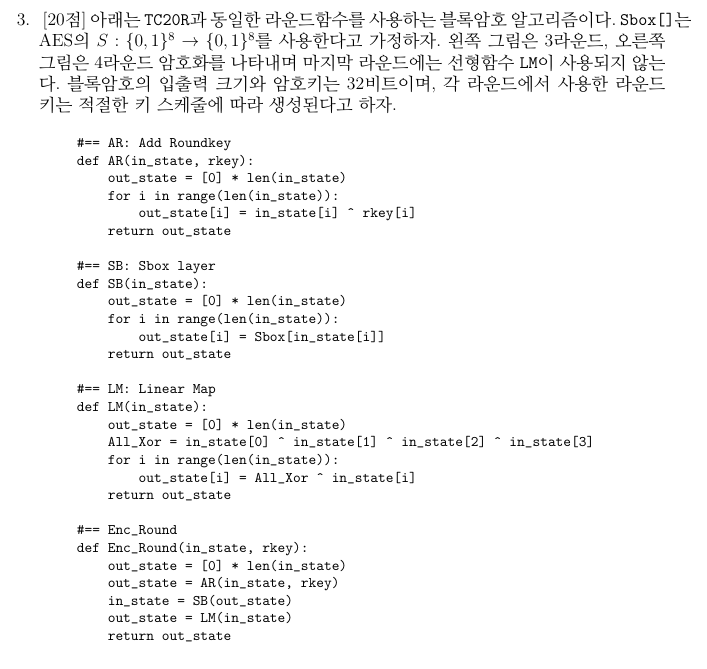
\includegraphics[scale=.5]{final2023-3}
		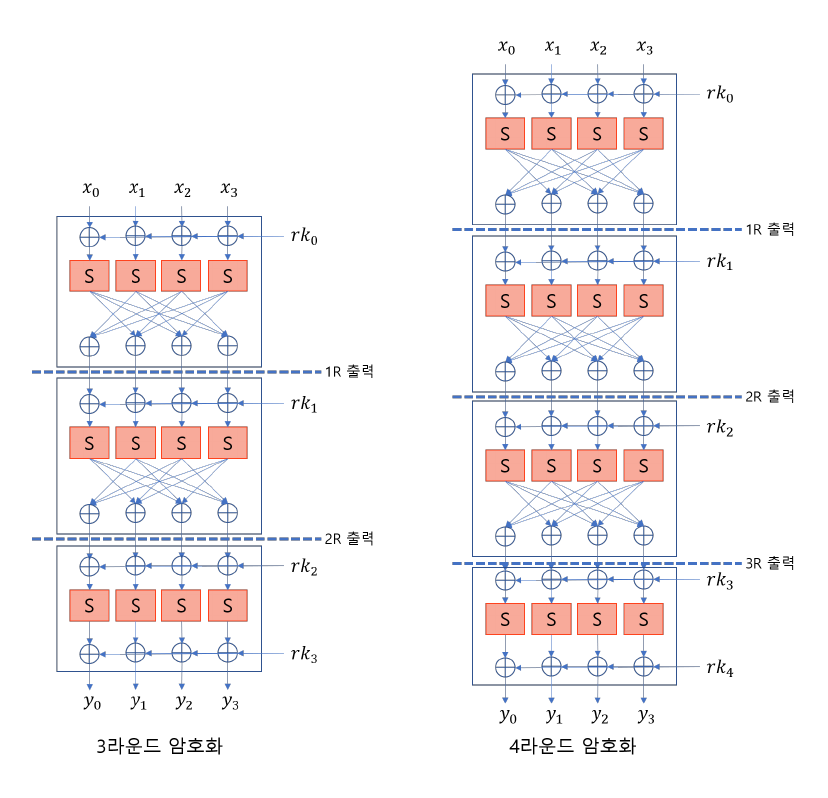
\includegraphics[scale=.375]{final2023-3-2}
	\end{figure}
	\begin{figure}[h!]\centering
		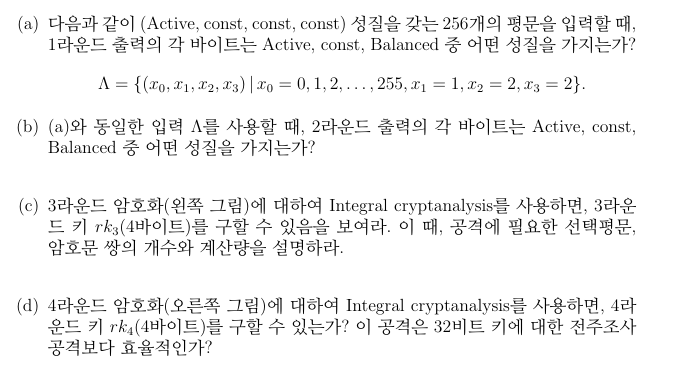
\includegraphics[scale=.55]{final2023-3-3}
	\end{figure}
	\begin{enumerate}[(a)]
		\item (1R) $(A,C,C,C)\xrightarrow{S}(A,C,C,C)\xrightarrow{LM}(C,A,A,A)$. Thus, \begin{center}
			(Const, Active, Active, Active)
		\end{center}
		\item (2R) $(C,A,A,A)\xrightarrow{S}(C,A,A,A)\xrightarrow{LM}(B,B,B,B)$. Thus, \begin{center}
			(Balanced, Balanced, Balanced, Balanced)
		\end{center}
		\item Blanced를 만족할 확률은 $1/2^8$이며, $2^8\times 1/2^8=1$이다. 따라서 $2^8=256$개만 하면 wrong key가 나올 수 있으니, $(P,C)$ 쌍 $2^8\times 2$ 개 정도 필요하다. Sbox 하나 당 \[
		2^8\times 2^8(\text{키후보})\times 2.
		\]
		\item 2라운드 0번째 바이트가 Balanced 인 것을 확인한다. \[
		rk_3'[0], rk_4[1], rk_4[2], rk_4[3]
		\]를 예측한다. 이는 $2^{32}$ 계산량으로 round key를 예측하는 것이므로 32 비트 ($2^{32}$) 키에 대한 전수보다 비효율적이다.
	\end{enumerate}
	\item[]
	\begin{figure}[h!]\centering
		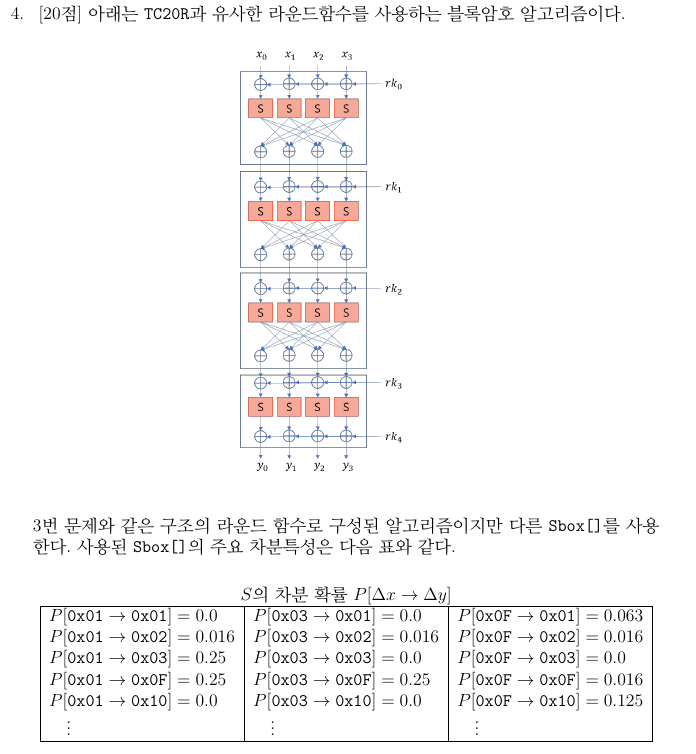
\includegraphics[scale=.6]{final2023-4}
		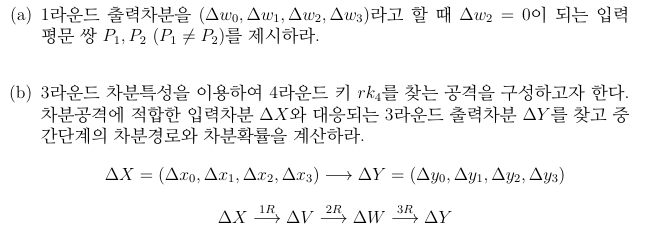
\includegraphics[scale=.6]{final2023-4-2}
	\end{figure}
	\newpage
	\begin{proof}[\sol]
		\ \begin{enumerate}[(a)]
			\item $P_1=\texttt{0x00\ 00\ 00\ 00}$, $P_2=\texttt{0x00\ 00\ 01\ 00}$
			\item Consider \begin{align*}
				(\alpha, 0, 0, 0)&\xrightarrow{S\ \text{with}\ p_1}(\beta,0,0,0)\quad\quad\cdots\cdots\ \text{Round 1}\\
				&\xrightarrow{LM}(0,\beta,\beta,\beta) \\ \\
				(0,\beta,\beta,\beta)&\xrightarrow{S\ \text{with}\ p_2^3}(0,\gamma,\gamma,\gamma)\quad\quad\cdots\cdots\ \text{Round 2}\\
				&\xrightarrow{LM}(\gamma,0,0,0)\\ \\
				(\gamma,0,0,0)&\xrightarrow{S\ \text{with}\ p_3^1}(\delta,0,0,0)\quad\quad\cdots\cdots\ \text{Round 3}\\
				&\xrightarrow{LM}(0,\delta,\delta,\delta)
			\end{align*} Consider \begin{align*}
				p_1=P[\texttt{0x01}\to\texttt{0x03}]&=0.25,\\
				p_2=P[\texttt{0x03}\to\texttt{0x0F}]&=0.25,\\
				p_3=P[\texttt{0x0F}\to\texttt{0x10}]&=0.125.
		\end{align*} Then $p=\displaystyle\left(\frac{1}{4}\right)\left(\frac{1}{4}\right)^3\left(\frac{1}{8}\right)=\frac{1}{2^{11}}>\frac{1}{2^{32}}$ and \begin{align*}
		(\texttt{0x01},\texttt{0x00},\texttt{0x00},\texttt{0x00})&\xrightarrow{1R}(\texttt{0x00},\texttt{0x03},\texttt{0x03},\texttt{0x03})\quad\quad\cdots\cdots\ p_1=1/4\\
		&\xrightarrow{2R}(\texttt{0x0F},\texttt{0x00},\texttt{0x00},\texttt{0x00})\quad\quad\cdots\cdots\ p_2^3=1/4^3\\
		&\xrightarrow{3R}(\texttt{0x00},\texttt{0x10},\texttt{0x10},\texttt{0x10})\quad\quad\cdots\cdots\ p_3=1/8.
	\end{align*}
		\end{enumerate}
	\end{proof}
	\newpage
	\item[]
	\begin{figure}[h!]\centering
	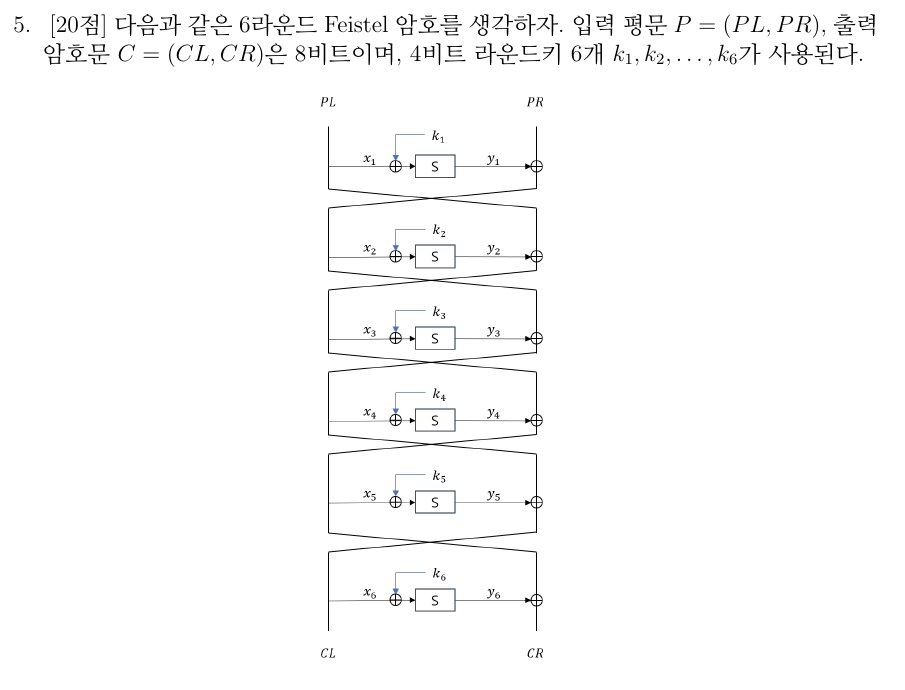
\includegraphics[scale=.45]{final2023-5}
	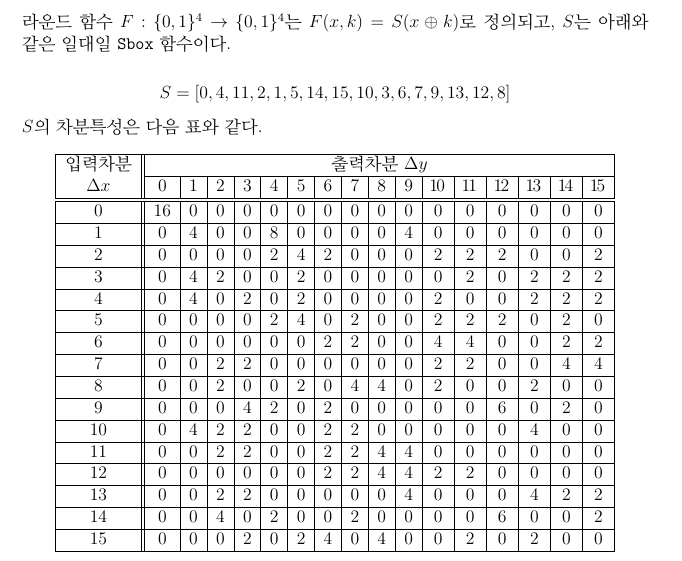
\includegraphics[scale=.55]{final2023-5-2}
	\end{figure}	
	\begin{figure}[h!]\centering
		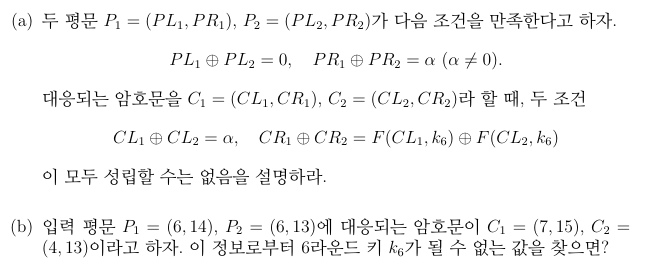
\includegraphics[scale=.55]{final2023-5-3}
	\end{figure}\
	\begin{proof}[\sol]
		\ \begin{enumerate}[(a)]
			\item 입력 차분 $(0,\alpha)$, 5라운드 차분 $(\alpha,0)$. 5R 불능차분특성: \[
			\alpha\oplus\alpha=0=\gamma\neq 0.
			\]
			\item Consider $\Delta P=P_1\oplus P_2=(0,14\oplus 13)=(0,3)$. Then\begin{itemize}
				\item $CL_1\oplus CL_2=7\oplus 4=3=\alpha$;
				\item $CR_1\oplus CR_2=F(CL_1,k_6)\oplus F(CL_2,k_6)$을 만족하는 $k_6$는 키 후보에서 삭제.
				\begin{itemize}
					\item $CR_1\oplus CR_2=15\oplus 3=2$
					\item \ \\ \adjustbox{scale=.9, center}{\begin{tabular}{c|cc|cc|c}
						$k_6$ & $0111\oplus k_6$ & $0100\oplus k_6$ & $S[0111\oplus k_6]$ & $S[0100\oplus k_6]$ & $\Delta=S[CL_1\oplus k_6]\oplus S[CL_2\oplus k_6]$ \\ \hline\hline
						$\vdots$ & $\vdots$ & $\vdots$ & $\vdots$ & $\vdots$ & $\vdots$ \\ \hline
						0100 & 0011 & 0000 & 0010 & 0000 & 0010
					\end{tabular}}
				\end{itemize}
			\end{itemize}\ \\ Thus, $k\neq 0100$
		\end{enumerate}
	\end{proof}
	\newpage
	\item[]
	\begin{figure}[h!]\centering
		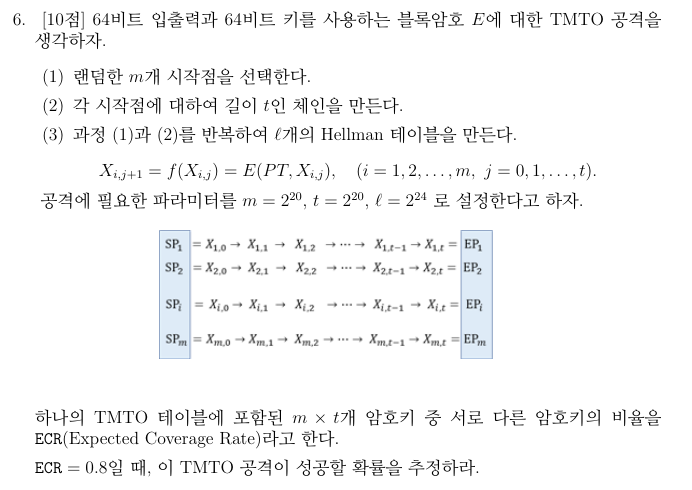
\includegraphics[scale=.55]{final2023-6}
	\end{figure}
	\begin{proof}[\sol]
		Note that \[
		\displaystyle 1-\left(1-\frac{ECR\cdot mt}{2^{64}}\right)^{\ell}.
		\] Since $(1-a)^b=\exp(-ab)$ ($\lim\limits_{h\to 0}(1+h)^{1/h}=e$, $\lim\limits_{a\to 0}(1-a)^b=\lim\limits_{a\to 0}[(1-a)^{-1/a}]^{-ab}=\exp(-ab)$), we have \[
		1-\exp(-\frac{ECR\cdot mt\ell}{2^{64}})=1-\exp(-0.8).
		\]
	\end{proof}
\end{enumerate}